% -*- coding: utf-8; -*-

\documentclass[
  phd,
  %% master
  brazilian
  %%american
]{ThesisPUC}


%%%
%%% Additional Packages
%%%

%%  \usepackage[brazilian]{babel}      %% in ThesisPUC.cls
  %% \usepackage[utf8]{inputenc}        %% .
  %% \usepackage[T1]{fontenc}           %% .
  %% \usepackage{lmodern}               %% .
  %% \usepackage[pdftex]{graphicx}	%% .

  \usepackage{tabularx}
  \usepackage{multirow}
  \usepackage{multicol}
  \usepackage{colortbl}
  \usepackage[%
    dvipsnames,
    svgnames,
    x11names,
    fixpdftex
  ]{xcolor}
  \usepackage{numprint}
  \usepackage{textcomp}
  \usepackage{booktabs}
  \usepackage{amsmath}
  \usepackage{enumitem}
  \usepackage{amssymb}
  \usepackage{textcomp}
% \usepackage{etoolbox}

%% numprint 
\npthousandsep{.}
\npdecimalsign{,}

%% ThesisPUC option
%\tablesmode{figtab} %% [nada, fig, tab ou figtab]
%\abreviationsmode{none} %% [none ou use] %% Default is [use]


%%%
%%% Counters
%%%

%% uncomment and change for other depth values
%% \setcounter{tocdepth}{3}
%% \setcounter{lofdepth}{3}
%% \setcounter{lotdepth}{3}
%% \setcounter{secnumdepth}{3}


%%%
%%% New commands and other global definitions
%%%

% -*- coding: iso-8859-1; -*-

%%%
%%% Newcommands
%%%

\newcommand{\degree}{\ensuremath{^\circ}}

\newcommand{\cetem}{Centro de Tecnologia Mineral}

\newcommand{\mybulletOB}{%
  % \textbullet
  % \checkmark
  $\triangleright$
  %\textopenbullet
}

\newcolumntype{L}{>{\raggedright \arraybackslash}X}
\newcolumntype{R}{>{\raggedleft \arraybackslash}X}
\newcolumntype{C}{>{\centering \arraybackslash}X}
\newcolumntype{M}[1]{>{\centering\hspace{0pt}}m{#1}}

\newcommand{\mrcel}[2]{%
\begin{tabular}[c]{@{}c@{}}#1\\#2\end{tabular}}

\newcommand{\mrcell}[2]{%
\begin{tabular}[l]{@{}l@{}}#1\\#2\end{tabular}}

\newcommand{\mrcelthree}[3]{%
\begin{tabular}[c]{@{}c@{}c@{}}#1\\#2\\#3\end{tabular}}

\newcommand{\mrcelcolorg}[2]{%
\begin{tabular}{l}\rowcolor{Gainsboro}#1\\#2\end{tabular}}

\newcommand{\mytbcimg}[3]{%
  \multicolumn{1}{C}{\parbox[c]{#1}{\includegraphics[width=#2]{#3}}}}


%%%
%%% Misc.
%%%

\usecolour{true}

%%%
%%% Titulos
%%%

\author{Wellington Carlos da Rosa Nascimento}
\authorR{Nascimento, Wellington Carlos da Rosa}

\advisor{Marco Aurélio Cavalcanti Pacheco}{Prof.}
\advisorR{Pacheco, Marco Aurélio Cavalcanti}
% If the advisor's department is different from author's department, uncomment the next line and type the correct name and acronym of advisor's institution.
%\advisorInst{institution name}{acronym}

\coadvisor{Marco Antonio Guimarães Dias}{Prof.}
\coadvisorR{Dias, Marco Antonio Guimarães}
\coadvisorInst{Departamento de Engenharia Elétrica}{PUC-Rio}

%% \title{Desenvolvimento de um sistema de microscopia digital para
%%  classificação automática de tipos de hematita em minério de ferro}

\title{Aplicação de Redes Neurais na Avaliação Econômica de Projetos de E\&P: Uma Abordagem Baseada em Valor da Informação Sequencial e Opções Reais}

\titleuk{Neural Networks Applied to the Economic Evaluation of E\&P Projects: A Sequential Value of Information and Real Options Approach}

%% \subtitulo{Aqui vai o subtitulo caso precise}

\day{07}
\month{Março}
\year{2025}

\city{Rio de Janeiro}
\CDD{620.11}
\department{Engenharia Elétrica}
\program{Engenharia Elétrica}
\school{Centro Técnico Científico}
\university{Pontifícia Universidade Católica do Rio de Janeiro}
\uni{PUC-Rio}

%%%
%%% Jury
%%%

\jury{%
  \jurymember{Pierre-Simon, Marquis de Laplace}{Prof.}
    {University of Caen}{France}
  \jurymember{Andrey Nikolaevich Kolmogorov}{Prof.}
    {Moscow State University}{Russian}
  \jurymember{William Sealy Gosset}{Prof.}
    {New College - Oxford}{England}
  \jurymember{Fischer Sheffey Black}{Prof.}
    {Harvard University}{USA}
}

%%%
%%% Resume
%%%

\resume{%
  Bacharel e Mestre em Física pela Universidade Federal de Alagoas. Trabalha desde de 2010 na Petrobras como Geofísico Senior atuando na Análise Econômica de Projetos Exploratórios.}

%%%
%%% Acknowledgment (REMINDER TO SCHOLARSHIP STUDENTS. Do not forget to thank the agencies that supported your work.)
%%%

\acknowledgment{%
  \noindent I would like to first thank my advisor testando...
  \bigskip

  \noindent Then I wish to thank ...
}

%%%
%%% Catalog prekeywords
%%%

\catalogprekeywords{%
  \catalogprekey{Engenharia Química}%
  \catalogprekey{Engenharia de Materiais}%
}

%%%
%%% Keywords
%%%

\keywords{%
  \key{Minério de Ferro}
  \key{Cristais de Hematita}
  \key{Microscopia Digital}
  \key{Análise de Imagens}
  \key{Classificação}
  \key{Microscopia de Luz Polarizada}
}

\keywordsuk{%
  \key{Iron Ore}%
  \key{Hematite Crystals}%
  \key{Digital Microscopy}%
  \key{Image Analysis}%
  \key{Classification}%
  \key{Polarized Light Microscopy}%
}

%%%
%%% Abstract
%%%

\abstract{%
  O minério de ferro é um material policristalino oriundo de processos
  naturais complexos durante tempos geológicos, que dão origem ...
}

\abstractuk{%
  Iron ore is a polycrystalline material created by complex natural
  processes during geological periods, which give rise to ...}

%%%
%%% Dedication
%%%

\dedication{%
  Aos meu pais, filhos e esposa. A todos os meus familiares.\\
À hipótese de Laplace.
}

%%%
%%% Epigraph
%%%

\epigraph{%
  My beautifull epigraph
}
\epigraphauthor{Wassily Kandinsky}
\epigraphbook{Regards sur le passé}

%%%
%%% Hyphenation
%%%

\hyphenation{PON-TI-FÍ-CIA}

%%%
%%% 
%%%

\begin{document}

  % -*- coding: utf-8; -*-

\chapter{Introduction}

This is the first chapter. In this chapter, let's have a nice image mais teste $\theta$  :


\begin{figure} [h]
  \begin{center}
    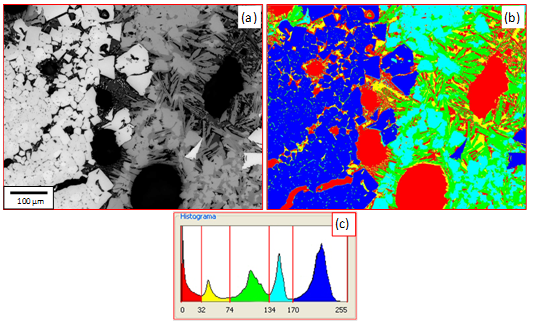
\includegraphics[height=243pt,width=400pt]{images/fig2-6}
    \caption{Example of thresholding: (a) original image; (b) processed
      image.\cite{74}}\label{fig:2-6}
  \end{center}
\end{figure}

  % -*- coding: utf-8; -*-

\chapter{Review}

This is the second chapter...

In this chapter, let's have a nice table:

%% -*- coding: utf-8; -*-

\begin{table} [!h]
  \caption{Principais minerais de ferro e suas classes.\cite{29}}\label{tab:2-4}
  ~\\[-1mm]
   \begin{tabularx}
     {\textwidth}
     { p{2.0cm}
       p{2.5cm}
       p{3.3cm}
       p{1.3cm}
       p{2.7cm}}

     \textbf{Classes}
     & \textbf{Minerais}
     & \textbf{\mrcel {Fórmula}{Química}}
     & \textbf{\mrcel{Teor}{de Fe}}
     & \textbf{\mrcel{~~Designação}{~~Comum}}
     \\\toprule

     ~ \\[-6mm]
     \multirow{5}{*}{Óxidos}& Magnetita
     & $Fe_{3}O_{4}$
     & ~72,4
     & \mrcel{~~Óxido ferroso}{~~férrico}
     \\%\midrule

     & Hematita
     & $Fe_{2}O_{3}$
     & ~69,9
     & ~~Óxido férrico \\[2mm]

     & Goethita
     & $FeO(OH)$
     & ~62,8
     & \multirow{2}{*}{\mrcel{Óxido-hidróxido}{de ferro}} \\[2mm]


     & Lepidocrocita
     & $FeO(OH)$
     & ~62,8 &
     \\\midrule

     Carbonato
     & Siderita
     & $FeCO_{3}$
     & ~48,2
     & \mrcel{~~~~Carbonato}{~~~~de Ferro}
     \\\midrule

     \multirow{2}{*}{Sulfetos}
     & Pirita
     & $FeS_{2}$
     & ~46,5
     & \multirow{2}{*}{~} \\[2mm]


     & Pirrotita
     & $FeS$
     & ~63,6
     & ~
     \\\midrule

     \multirow{10}{*}{Silicatos}
     & Fayalita
     & $Fe^{2+}_{2}(SiO_{4})$
     & ~54,8
     & \mrcel{~~~~Grupo da}{~~~~Olivina} \\[4mm]

     & Laihunite
     & $Fe^{2+}Fe^{3+}_{2}(SiO_{4})_{2}$
     & ~47,6
     & \mrcel{~~~~Grupo da}{~~~~Olivina} \\[4mm]

     & Greenalita
     & \mrcell{$2Fe^{2+}_{2}6Fe^{3+}Si_{2}$}{$4O_{5}(OH)_{3,3}$}
     & ~44,1
     & \mrcel{~~~~Grupo da}{~~~~Serpentina} \\[4mm]

     & Grunerita
     & \mrcell{$Fe^{2+}_{7}(Si_{8}O_{22})$}{$(OH)_{2}$}
     & ~39,0
     & \mrcel{~~~~Grupo dos}{~~~~Anfibólios} \\[4mm]

     & Fé-antofilita
     & \mrcell{$Fe^{2+}_{7}(Si_{8}O_{22})$}{$(OH)_{2}$}
     & ~39,0
     & \mrcel{~~~~Grupo dos}{~~~~Anfibólios}
     \\\midrule
   \end{tabularx}
\end{table}


\section{Hematite}

A hematita é o mineral de ferro mais importante devido a sua alta
ocorrência em vários tipos de rochas e suas origens diversas.\cite{30}
A composição química deste mineral é Fe$_{2}$O$_{3}$, com uma fração
mássica em ferro de 69,9\% e uma fração mássica em oxigênio de
30,1\%.\cite{31}

...


\subsection{Martite}

A hematita é o mineral de ferro mais importante devido a sua alta
ocorrência em vários tipos de rochas e suas origens diversas.\cite{30}
A composição química deste mineral é Fe$_{2}$O$_{3}$, com uma fração
mássica em ferro de 69,9\% e uma fração mássica em oxigênio de
30,1\%.\cite{31}

...


\subsubsection{Globular}

A hematita é o mineral de ferro mais importante devido a sua alta
ocorrência em vários tipos de rochas e suas origens diversas.\cite{30}
A composição química deste mineral é Fe$_{2}$O$_{3}$, com uma fração
mássica em ferro de 69,9\% e uma fração mássica em oxigênio de
30,1\%.\cite{31}

...

\subsubsection{Escaping percent in a title:  100\%}

  % -*- coding: utf-8; -*-

\chapter{Conclusions}

Um sistema de microscopia digital com reconhecimento e classificação
automática dos cristais de hematita em minérios de ferro foi
desenvolvido.

O método utiliza operações tradicionais de processamento digital de
imagens e propõe uma segmentação automática de cristais baseada no
cálculo da distância espectral, a fim de controlar ...

É fundamental também comentar que ...

Assim, como uma proposta para trabalho futuro, pode-se buscar combinar
os dois enfoques...

  %% ...
  \arial
  \bibliography{tiny}
  \normalfont
  % -*- coding: utf-8; -*-

\appendix
\chapter{Published paper}

The following paper was published ...

\end{document}
